%Préambule du document :
\documentclass[12pt, a4paper]{book}
%\usepackage[latin1]{inputenc} 
\usepackage[utf8]{inputenc} % accents
\usepackage{gensymb} % degree symbol ° (\degree)
\usepackage[T1]{fontenc} % | "`pipe"' character
\usepackage{graphicx}
\usepackage{titling}
\usepackage{amssymb} 
\usepackage{minitoc} % chapter's tocs
\usepackage{authblk} % author affiliations
\usepackage{fancyhdr} % modify the headers
\usepackage{tabularx} % tables not larger than A4
\usepackage[table]{xcolor} %colors inside the tables
\usepackage{float}
\usepackage{multicol} % multiple columns in some sections
\usepackage[inner=2cm,outer=2cm]{geometry} %A4 margins
\usepackage{siunitx}
\usepackage[labelfont=bf, margin=0.5cm]{caption} % for figure captions in minipages
\usepackage{hyperref} %link references (toc, citations) inside document
\usepackage{natbib} % to cite with parentheses and plain text et only year if you please...
\usepackage{amsmath}
 \usepackage{fixltx2e} % allows overrightarrow to be in caption

\hyphenation{Cur-vature} %Example of hyphenation

 \MakeRobust{\overrightarrow}


\bibliographystyle{plainnat} % reference style
\renewcommand{\bibname}{References} %Rename "`bibliography"' => "`references"'
\newcommand*{\doi}[1]{\href{https://doi.org/#1}{doi: #1}}


\hypersetup{
    colorlinks,
    citecolor=brown,
    filecolor=green,
    linkcolor=red,
    urlcolor=blue
}
\hypersetup{linktocpage}


\pagestyle{fancy}
\fancyhead{}
\fancyfoot{}
\fancyhead[RO,LE]{\thepage}
\fancyhead[LO]{\leftmark}
\fancyhead[RE]{\rightmark}
\setcounter{tocdepth}{1} % we only want chapters and sections in toc
\setcounter{minitocdepth}{2} %we want sections and subsections in chapters' minitocs

\pretitle{%
  \begin{center}
  
  
\includegraphics[width=17cm]{../Logo_software.png}\\[\bigskipamount]
}
\posttitle{
\\
  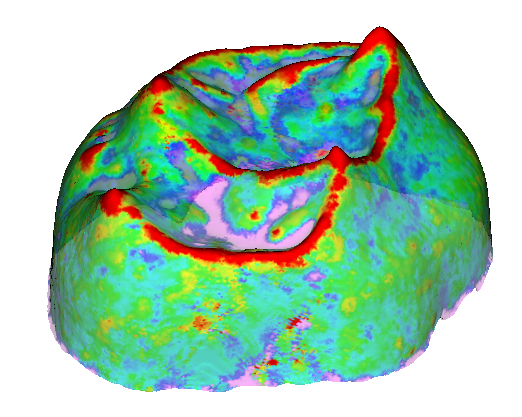
\includegraphics[width=8cm]{tutorial09.png}\\[\bigskipamount]
\end{center}}

%\postdate{
%
\includegraphics[width=15cm]{logo_affiliations.png}
%}

\title{Tutorial 09: curvature, scalar smoothing and normalization}



%\titlepicture[width=13cm]{Logo_software.png}
\author{Renaud LEBRUN}
\affil{Institut des Sciences de l'Evolution, Université de Montpellier, France}
\date{\today} 

\def\chaptername{Tutorial}
\setcounter{chapter}{9}
%Corps du document :
\begin{document}

	\dominitoc

\maketitle


\faketableofcontents

%\chapter{Working with landmarks}
\addstarredchapter{curvature, scalar smoothing and normalization}

\markboth{Tutorial 09: curvature, scalar smoothing and normalization}{}

\minitoc 
Tutorial 09 includes:
\begin{itemize}
\item One .ntw (MorphoDig project) file
\item One .vtk surface file representing the Enamel Dentine Junction (EDJ) of a Neolithic human upper left second molar.
\item One .pos (position) files 
\item The present .pdf document
\end{itemize}



\section{About the specimen}
The 3D model corresponds to a virtually reconstructed Enamel-Dentine Junction (EDJ) of a left upper permanent second molars (LUM2) from a Neolithic human of the necropolis of Gurgy (France). This specimen (GLN04-201-ULM2) was published in \citet{LeLuyer2016}, and the 3D model was released in \citet{LeLuyer2016a}.
The 3D data were obtained by computerized microtomography at the MRI \si{\micro}CT platform housed at the ISEM. 


\section{A brief overview of enclosed files}
		
The present tutorial contains a project .ntw file, which is useful to open the EDJ surface in a convenient position. Open the enclosed .ntw file (File->Open Project, then select "Curvature\_smoothing\_normalization.ntw"). Once loaded, the surface is opened and given a position and a color. Note that the newly opened surface is unselected.


\section{Tutorial}

\subsection{Curvature}
The EDJ 3D representation already contains 4 "Curvature" scalar arrays: Curvature\_mean, Curvature\_min, Curvature\_max, Curvature\_gaussian.\\ 
The curvature dialog can be opened by clicking on Scalars->Compute curvature for each selected surface (see Fig. \ref{curvature_dialog} p.\pageref{curvature_dialog}). These arrays were computed using the vtkCurvatures filter.\\
The vtkCurvatures filter offers 4 ways to compute surface's
curvature at each vertex. :\\
- Principal maximal curvature\\
- Principal minimal curvature\\
- Gaussian curvature\\
- Mean curvature.\\

\begin{figure}
  \centering
  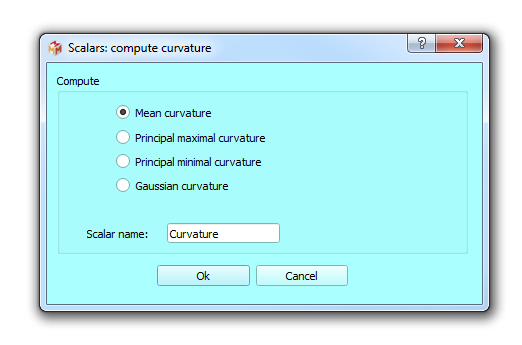
\includegraphics[scale=0.5]{curvature_dialog.png} 
	\caption{Curvature dialog.}
\label{curvature_dialog}
\end{figure}

\subsection{Smoothing}
The 4 "Curvature" scalar arrays (Curvature\_mean, Curvature\_min, Curvature\_max, Curvature\_gaussian) contain a lot of noise. In order to reduce noise and retrieve more biologically relevant information, scalars can be "smoothed" in different ways (see \ref{smoothing_scalars_dialog}). In our case, for each vertex, all "vertices closer than surface average size/40" were retrieved, and the smooth output was computed as the median of the scalar values found for all found neighbor vertices.

\begin{figure}
  \centering
  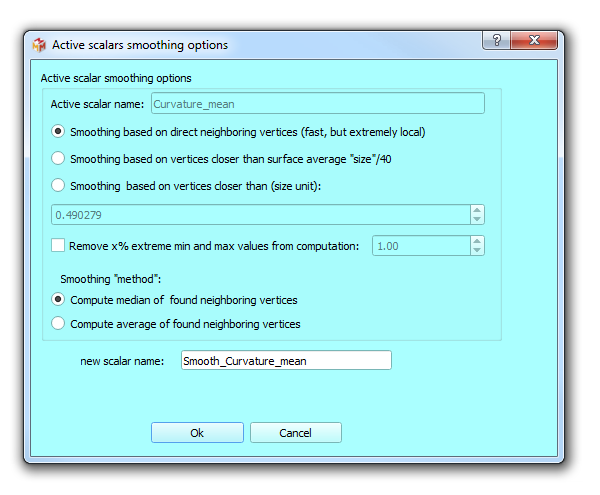
\includegraphics[scale=0.5]{scalar_smoothing_dialog.png} 
	\caption{ 
Scalar smoothing dialog. Smoothing can be computed using only direct neighbor vertices. Here, for each vertex, a much larger area was investigated to produce a "smoothed" output: smoothing was based on vertices closer than surface average size/40. The output was computed as the as the median of the scalar values found for the neighbor vertices.
	}
\label{smoothing_scalars_dialog}
\end{figure}

\subsection{Normalization}
In this case, it may be useful to normalize scalar values between 0 and 1, as the 4 smoothed scalar arrays (Smooth\_Curvature\_mean, Smooth\_Curvature\_max, Smooth\_Curvature\_min and Smooth\_Curvature\_gaussian) have very different min-max ranges. Doing so, we will make it possible to compare qualitatively these 4 scalar arrays using a unique color scale ranging between 0 and 1. The scalar normalization dialog was opened ("Scalars->Normalize or rescale active scalars for each selected surface", Fig. \ref{normalization_dialog} p.\pageref{normalization_dialog}), and for each of the 4 smoothed scalar arrays, 5\% scalars most extreme values were removed. Now, the 4 normalized smoothed arrays (Norm\_Smooth\_Curvature\_mean, Norm\_Smooth\_Curvature\_max etc.) can be directly compared qualitatively (Fig. \ref{normalization_example} p.\pageref{normalization_example}).

\begin{figure}
  \centering
  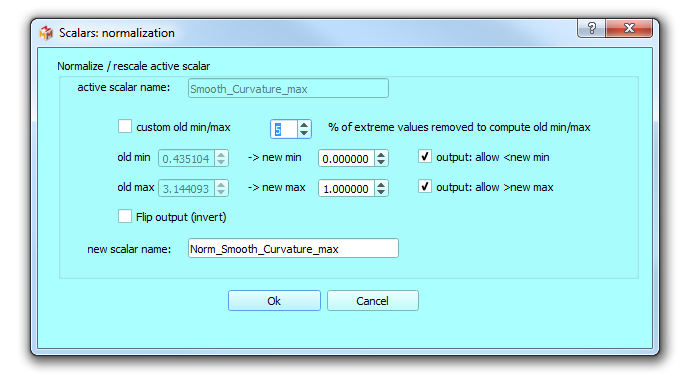
\includegraphics[scale=0.5]{normalization_dialog.png} 
	\caption{ 
Scalar normalization/rescale dialog. The "old min" and "old max" value represent by default the minimal and maximal value of the active scalars within \textbf{all} currently opened surfaces. After the scalar normalization/rescale has been performed, "old min" will have been set to "new min", "old max" will have been set to "new max", and scalar values in between "old min" and "old max" will range between "new min" and "new max" using a linear interpolation. "old min" and "old max" can be given other values than the real min and max of the active scalar via two options. \textbf{1)} a given percentage of extreme min and max values can be removed from the current active scalar values (sometimes only a few extreme "strange" values can give a wrong idea of the "real" extant of the range of a given scalar). This is the option chosen in this tutorial. \textbf{2)} if the "custom old min/max" option is checked, old min and old max values can be set to any value.  When one of these two options is used, the interpolated values produced may fall above "new max" or below "new min". Then you may decide whether you allow such "out of the range" values using the "allow < new min" and "allow > new max" options. If unchecked, interpolated values falling below "new min" will be set to "new min", and interpolated values falling above "new max" will be set to "new max". The "flip output" option will reverse the range of interpolated values between "new min" and "new max".
	}
\label{normalization_dialog}
\end{figure}

\begin{figure}
  \centering
  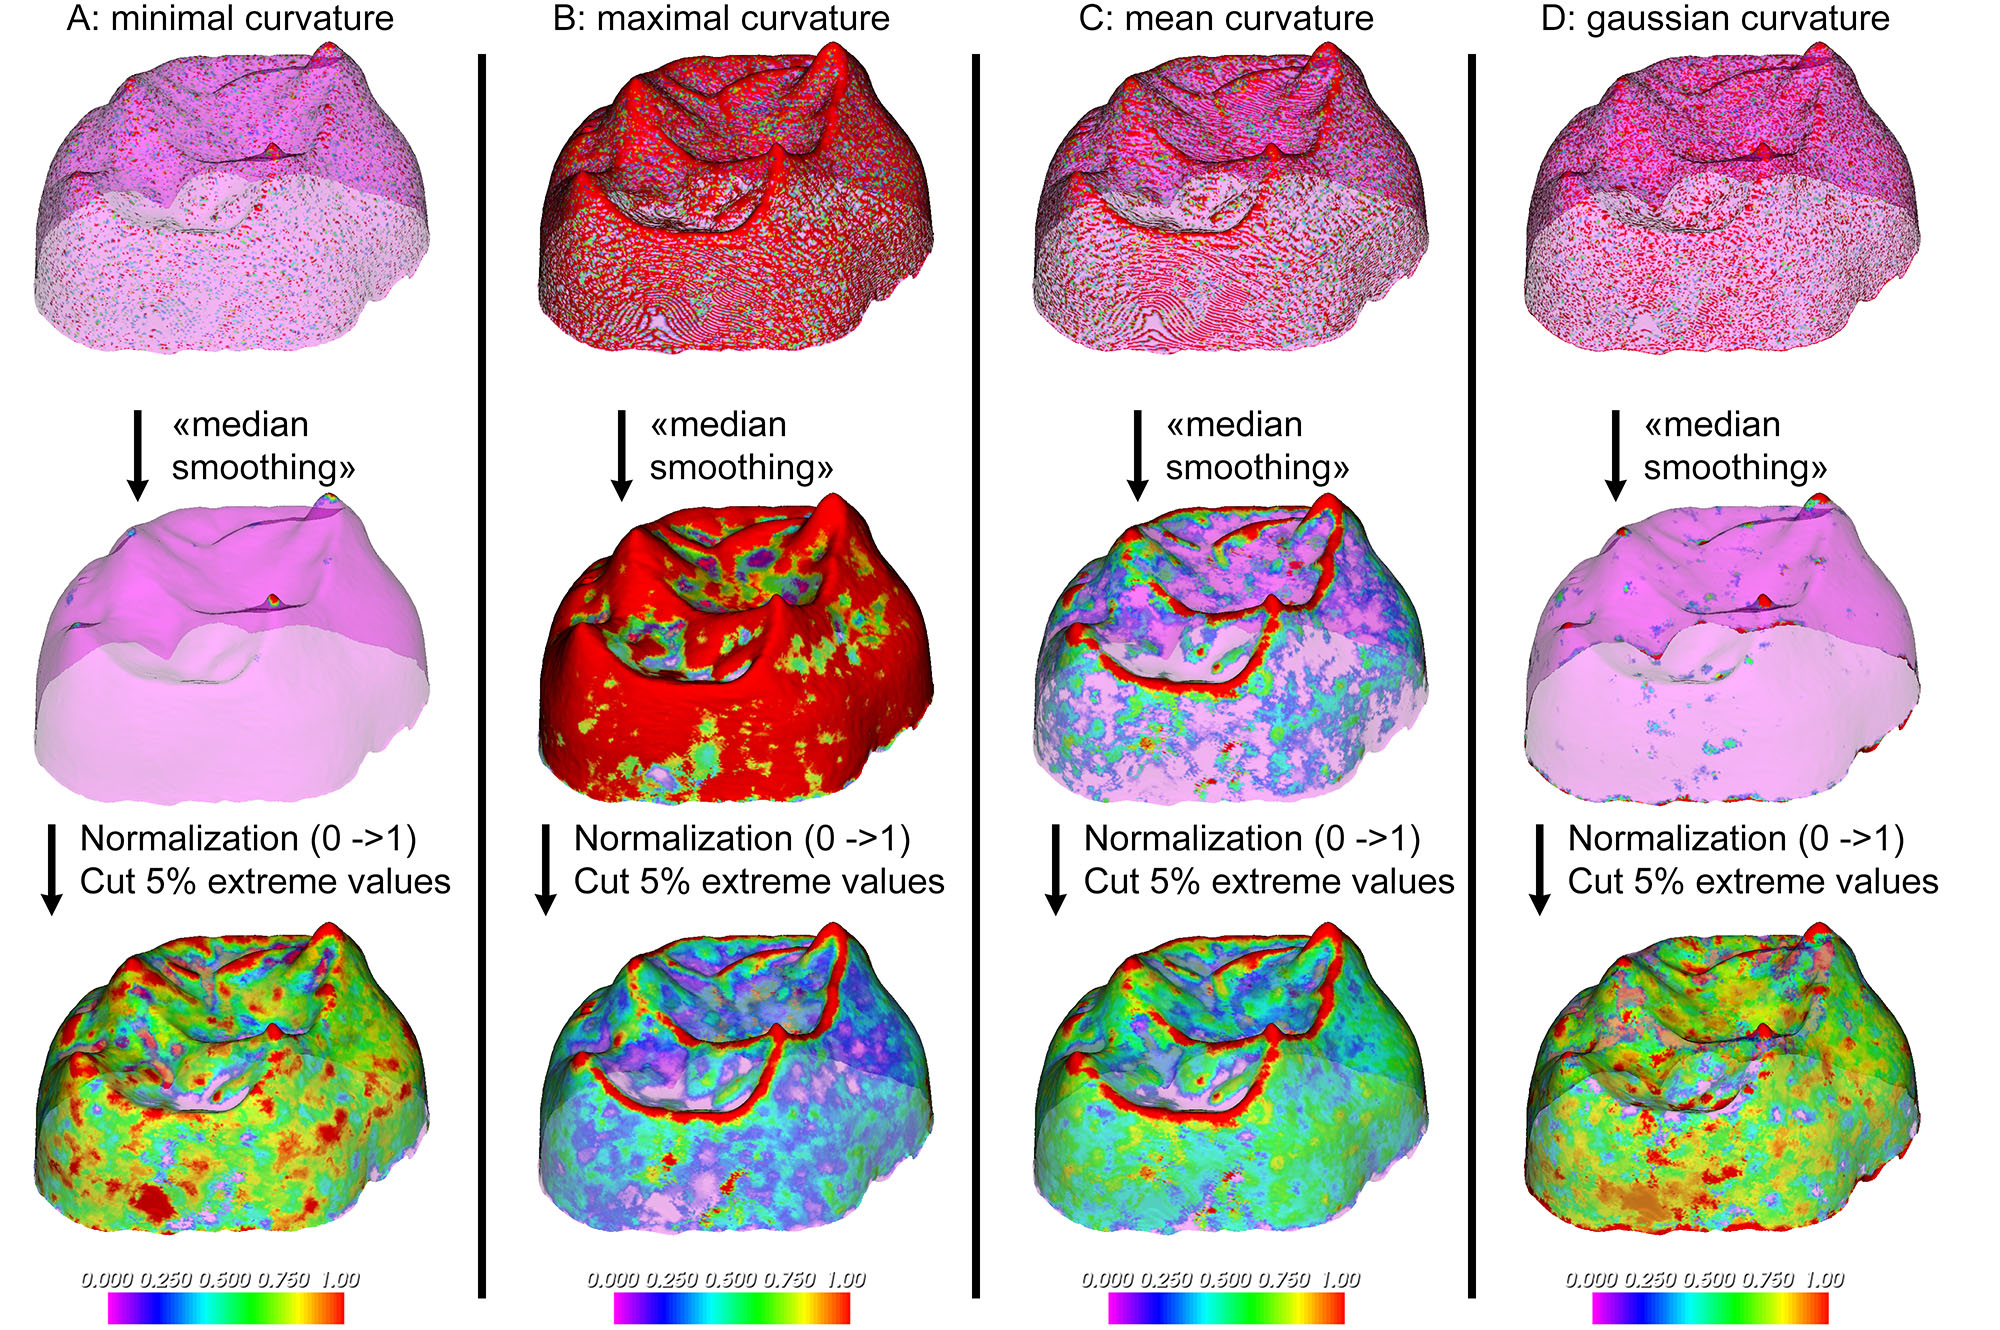
\includegraphics[scale=0.26]{normalization_example.jpg} 
	\caption{ 
Normalization of different scalars within the same surface. All illustrations use the same color table, ranging between 0 and 1.  \textbf{A} : "Minimal curvature".  \textbf{B} : "Maximal curvature". \textbf{C} : "Mean curvature". \textbf{D} : "Gaussian curvature". Top line: "raw" 4 scalars, which all express a lot of noise. Middle line: the 4 same "smoothed"' scalars after a median filter has been used. Bottom line: the 4 same scalars after normalization. The 5\% most extreme minimal values and maximal values have been excluded from this normalization process, because they are clearly aberrant (most values range between -10 and 10 for all 4 raw scalars, but a few outliers have values above 10000 and below -10000). The visual output of the bottom line is easier to interpret.	
	}
\label{normalization_example}
\end{figure}

\section{Acknowledgements}
MicroCT data acquisition was funded by the Research National Agency through the DHP project (dir: S. Rottier; 2012-14; Université Bordeaux 1/LaScArBx; Grant number: ANR-10-LABX-52) and the PEPS 3Dent’in (dir: P. Bayle; 2013-14; PEPS IdEx Bordeaux/CNRS; Grant number: ANR-10-IDEX-03-02). M. Le Luyer, who performed 3D data acquisition, benefited from a doctoral grant of the Ministère de l’Enseignement Supérieur et de la Recherche. MicroCT data presented in this work were produced through the technical facilities of the MRI platform and of the labEx CeMEB.


%\nocite{*}   % All bibliography items appear without citation in the text

%\cleardoublepage
%\phantomsection

\addcontentsline{toc}{section}{References}
\bibliography{References}	

\end{document} 

